\documentclass[10pt,a4paper]{article}
\usepackage[margin=1.7cm]{geometry}
\usepackage[T1]{fontenc}
\usepackage{lmodern}
\usepackage{xcolor}
\usepackage{booktabs}
\usepackage{array}
\usepackage{colortbl}
\usepackage{amsmath}
\usepackage{amssymb}
\usepackage{enumitem}
\usepackage{tabularx}
\usepackage{mdframed}
\usepackage{tikz}
\usepackage{pgfplots}
\pgfplotsset{compat=1.17}
\usetikzlibrary{positioning,arrows.meta,fit,backgrounds,shapes.geometric,calc}
\usepackage[colorlinks=true]{hyperref}

% ── Palette (shared with the rest of docs/) ───────────────────────────────────
\definecolor{hdrblue}{RGB}{10,60,140}
\definecolor{accentteal}{RGB}{0,120,120}
\definecolor{okgreen}{RGB}{20,110,40}
\definecolor{passrowbg}{RGB}{220,245,225}
\definecolor{badred}{RGB}{180,20,20}
\definecolor{warnamber}{RGB}{180,90,0}
\definecolor{newbg}{RGB}{210,235,255}
\definecolor{newtext}{RGB}{0,60,130}
\definecolor{rulegray}{RGB}{130,130,130}
\definecolor{tablegray}{RGB}{245,246,248}
\definecolor{hwfill}{RGB}{222,236,255}
\definecolor{swfill}{RGB}{255,238,214}
\definecolor{goldfill}{RGB}{255,247,210}

\hypersetup{linkcolor=hdrblue, urlcolor=accentteal,
  pdftitle={FPGA Tick-to-Trade: Complete Project Flow}}

\setlength{\parindent}{0pt}
\setlength{\parskip}{4pt}

\newcommand{\sectionrule}{\par\nobreak\vspace{1pt}\textcolor{rulegray}{\rule{\linewidth}{0.8pt}}\par\vspace{1pt}}
\newcommand{\fpath}[1]{\texttt{\textcolor{hdrblue}{#1}}}

\newmdenv[linecolor=newtext, backgroundcolor=newbg, linewidth=1.2pt,
  leftmargin=0pt, rightmargin=0pt, innerleftmargin=8pt, innerrightmargin=8pt,
  innertopmargin=6pt, innerbottommargin=6pt, skipabove=6pt, skipbelow=6pt]{keybox}

% ── TikZ node styles ──────────────────────────────────────────────────────────
\tikzset{
  hw/.style   ={rectangle, rounded corners=2pt, draw=hdrblue, fill=hwfill,
                text width=2.5cm, align=center, font=\footnotesize, minimum height=0.9cm, thick},
  sw/.style   ={rectangle, rounded corners=2pt, draw=warnamber, fill=swfill,
                text width=2.5cm, align=center, font=\footnotesize, minimum height=0.9cm, thick},
  gold/.style ={rectangle, rounded corners=2pt, draw=accentteal, fill=goldfill,
                text width=2.5cm, align=center, font=\footnotesize, minimum height=0.9cm, thick},
  src/.style  ={rectangle, rounded corners=2pt, draw=rulegray, fill=tablegray,
                text width=2.4cm, align=center, font=\footnotesize, minimum height=0.9cm},
  flow/.style ={-{Stealth[length=2.2mm]}, thick, draw=hdrblue},
  flowg/.style={-{Stealth[length=2.2mm]}, thick, draw=accentteal, dashed},
}

\begin{document}

% ── Title ─────────────────────────────────────────────────────────────────────
{\LARGE\bfseries\color{hdrblue} FPGA Tick-to-Trade \textendash{} Complete Project Flow}%
\hfill{\small\color{rulegray} 17 June 2026}\\[-2pt]
{\large\color{accentteal} From a market message to a trade, in nanoseconds \textendash{} and why hardware wins}

\textcolor{hdrblue}{\rule{\linewidth}{2pt}}

\begin{keybox}
{\large\bfseries\color{newtext} What this project is}

\smallskip
A high-frequency trading \emph{tick-to-trade} engine built in \textbf{RTL
(SystemVerilog)} for an AWS F1 (Xilinx UltraScale+ VU9P) FPGA. It ingests a
market-data feed, maintains a live order book, computes a trading signal, runs
pre-trade risk checks, and emits an order \textbf{entirely in hardware} --- a
measured \textbf{205\,ns} (41 clock cycles @ 200\,MHz). The same logic is
mirrored bit-for-bit in Python both as a verification golden model and as the
live software trading path, so the hardware speed can be measured against a
real software baseline on real market data.

\smallskip
\textbf{The thesis:} a deeply pipelined spatial dataflow in silicon does in
205\,ns what a software stack + broker network does in milliseconds --- a
$\sim$10{,}000\texttt{--}100{,}000$\times$ gap. This document walks the entire
flow and explains every file.
\end{keybox}

% ── 1. System architecture ─────────────────────────────────────────────────────
{\large\bfseries\color{hdrblue} 1.\quad System Architecture \textendash{} The Two Paths}
\sectionrule

The project is organised around a \textbf{dual path}. The \textcolor{hdrblue}{\textbf{fast
(hardware) path}} is the FPGA pipeline that is the engineering centrepiece. The
\textcolor{warnamber}{\textbf{slow (software) path}} mirrors the identical logic on a host CPU and routes
to a real paper broker, providing both a correctness oracle and the latency
baseline to beat.

\vspace{4pt}
\begin{center}
\resizebox{\linewidth}{!}{%
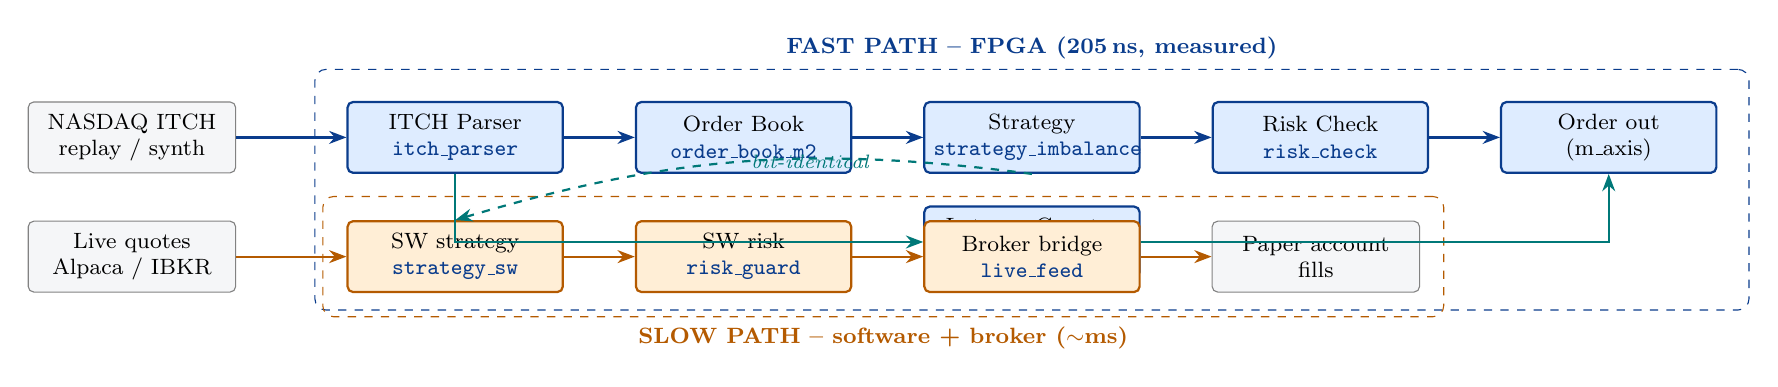
\begin{tikzpicture}[node distance=6mm and 9mm]
% sources
\node[src] (itch)  {NASDAQ ITCH\\ replay / synth};
\node[src,below=of itch] (live) {Live quotes\\ Alpaca / IBKR};

% hardware pipeline
\node[hw, right=14mm of itch] (parser) {ITCH Parser\\ \fpath{itch\_parser}};
\node[hw, right=of parser] (book)   {Order Book\\ \fpath{order\_book\_m2}};
\node[hw, right=of book]   (strat)  {Strategy\\ \fpath{strategy\_imbalance}};
\node[hw, right=of strat]  (risk)   {Risk Check\\ \fpath{risk\_check}};
\node[hw, right=of risk]   (out)    {Order out\\ (m\_axis)};
\node[hw, below=4mm of strat] (lat) {Latency Counter\\ \fpath{latency\_counter}};

% software path
\node[sw, right=14mm of live] (sws) {SW strategy\\ \fpath{strategy\_sw}};
\node[sw, right=of sws] (swr) {SW risk\\ \fpath{risk\_guard}};
\node[sw, right=of swr] (brk) {Broker bridge\\ \fpath{live\_feed}};
\node[src, right=of brk] (paper) {Paper account\\ fills};

% flows hardware
\draw[flow] (itch) -- (parser);
\draw[flow] (parser) -- (book);
\draw[flow] (book) -- (strat);
\draw[flow] (strat) -- (risk);
\draw[flow] (risk) -- (out);
\draw[flow, draw=accentteal] (parser.south) |- (lat.west);
\draw[flow, draw=accentteal] (lat.east) -| (out.south);
% flows software
\draw[flow, draw=warnamber] (live) -- (sws);
\draw[flow, draw=warnamber] (sws) -- (swr);
\draw[flow, draw=warnamber] (swr) -- (brk);
\draw[flow, draw=warnamber] (brk) -- (paper);
% equivalence link
\draw[flowg] (strat.south) to[bend right=12] node[midway,right,font=\scriptsize\itshape,text=accentteal]{bit-identical} (sws.north);

\begin{scope}[on background layer]
  \node[fit=(parser)(out)(lat), draw=hdrblue, dashed, rounded corners,
        inner sep=4mm, label={[hdrblue,font=\footnotesize\bfseries]above:FAST PATH \textendash{} FPGA (205\,ns, measured)}] {};
  \node[fit=(sws)(paper), draw=warnamber, dashed, rounded corners,
        inner sep=3mm, label={[warnamber,font=\footnotesize\bfseries]below:SLOW PATH \textendash{} software + broker ($\sim$ms)}] {};
\end{scope}
\end{tikzpicture}}
\end{center}

\begin{keybox}
\textbf{Why two paths?} The FPGA cannot legally sit in a retail broker's
critical order path, and raw NASDAQ ITCH is not retail-accessible. So the FPGA's
205\,ns is reported as a \emph{measured compute benchmark}; the live software
path (which \emph{is} bit-identical to the hardware) trades real paper orders and
supplies the apples-to-apples baseline. \textbf{Same decisions, two substrates,
one latency comparison.}
\end{keybox}

% ── 2. The hardware pipeline in detail ─────────────────────────────────────────
{\large\bfseries\color{hdrblue} 2.\quad The Hardware Pipeline \textendash{} Stage by Stage}
\sectionrule

Each stage is a dedicated circuit; data flows through them like a factory line.
Because every stage works \emph{simultaneously} on a different message, the
pipeline sustains one message per cycle while any single message clears in
41 cycles.

\vspace{3pt}
\begin{center}
\resizebox{\linewidth}{!}{%
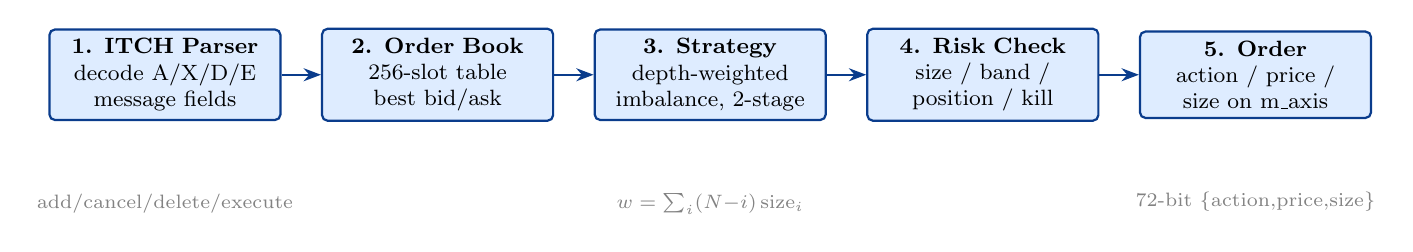
\begin{tikzpicture}[node distance=5mm]
\node[hw, text width=2.7cm] (a) {\textbf{1. ITCH Parser}\\ decode A/X/D/E\\ message fields};
\node[hw, text width=2.7cm, right=of a] (b) {\textbf{2. Order Book}\\ 256-slot table\\ best bid/ask};
\node[hw, text width=2.7cm, right=of b] (c) {\textbf{3. Strategy}\\ depth-weighted\\ imbalance, 2-stage};
\node[hw, text width=2.7cm, right=of c] (d) {\textbf{4. Risk Check}\\ size / band /\\ position / kill};
\node[hw, text width=2.7cm, right=of d] (e) {\textbf{5. Order}\\ action / price /\\ size on m\_axis};
\foreach \x/\y in {a/b,b/c,c/d,d/e} \draw[flow] (\x) -- (\y);
\node[below=8mm of a.south, font=\scriptsize, text=rulegray] {add/cancel/delete/execute};
\node[below=8mm of c.south, font=\scriptsize, text=rulegray] {$w=\sum_i (N{-}i)\,\text{size}_i$};
\node[below=8mm of e.south, font=\scriptsize, text=rulegray] {72-bit \{action,price,size\}};
\end{tikzpicture}}
\end{center}

\textbf{How the imbalance signal works.} The strategy weights the top
$N{=}4$ book levels by depth ($w=\sum_i (N{-}i)\cdot\text{size}_i$; the touch
counts heaviest) and fires using a division-free cross-multiply:
\[
\text{BUY if } w_{\text{bid}}\cdot 10 > \text{THRESH}\cdot w_{\text{ask}},
\qquad
\text{SELL if } w_{\text{ask}}\cdot 10 > \text{THRESH}\cdot w_{\text{bid}}.
\]
\texttt{THRESH}=15 means a \textbf{1.5$\times$} volume imbalance. The same ratio
scales the order lot (1$\times$/2$\times$/3$\times$ a base lot, capped). A spread
guard, a 2-consecutive-cycle validity gate, and an 8-cycle cooldown prevent
spurious fires. \textbf{No floating point} anywhere --- prices are integers in
units of $1/10{,}000$\,USD, matching the ITCH wire format.

\textbf{How latency is measured (in hardware).} \fpath{latency\_counter} latches
$t_0$ at message-start and $t_1$ when the decision appears, accumulating
$\Delta=t_1-t_0$ into a 64-bucket histogram readable over AXI-Lite (address map
in \fpath{f1/register\_map.md}). The headline result: \textbf{41 cycles =
205\,ns} at 200\,MHz.

% ── 3. Data collection ─────────────────────────────────────────────────────────
{\large\bfseries\color{hdrblue} 3.\quad How Data Is Collected \textendash{} Three Feeds}
\sectionrule

The exact same parser/book/strategy logic is exercised by three progressively
more realistic data sources:

\vspace{3pt}
\begin{center}
\resizebox{\linewidth}{!}{%
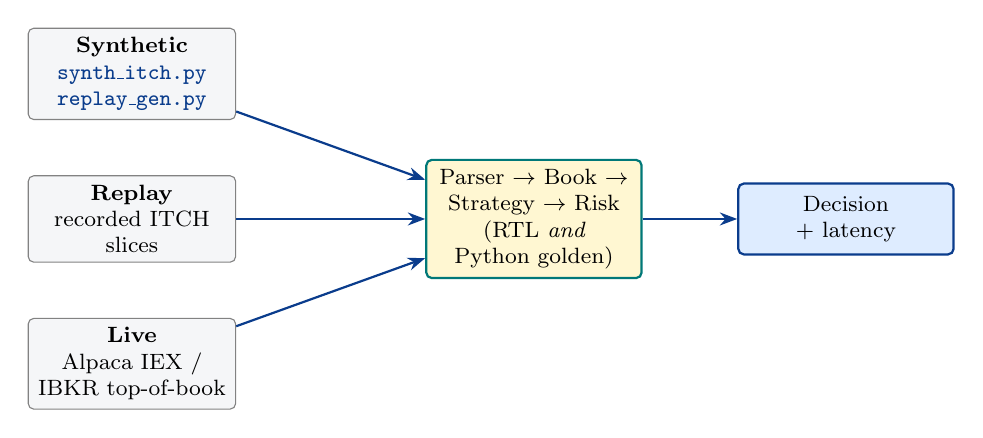
\begin{tikzpicture}[node distance=7mm and 12mm]
\node[src] (syn) {\textbf{Synthetic}\\ \fpath{synth\_itch.py}\\ \fpath{replay\_gen.py}};
\node[src, below=of syn] (rep) {\textbf{Replay}\\ recorded ITCH\\ slices};
\node[src, below=of rep] (liv) {\textbf{Live}\\ Alpaca IEX /\\ IBKR top-of-book};
\node[gold, right=24mm of rep] (eng) {Parser $\to$ Book $\to$ Strategy $\to$ Risk\\ (RTL \emph{and} Python golden)};
\node[hw, right=of eng] (dec) {Decision\\ + latency};
\foreach \s in {syn,rep,liv} \draw[flow] (\s) -- (eng);
\draw[flow] (eng) -- (dec);
\end{tikzpicture}}
\end{center}

\begin{itemize}[leftmargin=1.4em, topsep=2pt, itemsep=1pt]
\item \textbf{Synthetic} --- seeded ITCH generators build a realistic book
  (\fpath{sim/synth\_itch.py}, \fpath{sim/replay\_gen.py}) for deterministic,
  repeatable tests.
\item \textbf{Replay} --- recorded ITCH slices feed the parser to validate book
  reconstruction against the golden model over large message runs.
\item \textbf{Live} --- \fpath{host/live\_feed.py} streams real top-of-book
  quotes (Alpaca free IEX, or IBKR) into the software mirror; the
  \texttt{-{}-simulate} mode uses \fpath{host/quote\_sim.py} for an offline
  continuous feed. \emph{Live equities feeds are normalised top-of-book, not raw
  ITCH} --- the FPGA's ITCH parser is exercised by the synthetic/replay paths,
  the live path drives the bit-identical software strategy.
\end{itemize}

% ── 4. Why the FPGA is faster ───────────────────────────────────────────────────
{\large\bfseries\color{hdrblue} 4.\quad Why the Hardware Is Faster}
\sectionrule

\begin{minipage}[t]{0.50\linewidth}
A CPU executes the pipeline \emph{temporally}: fetch/decode/execute each
instruction of the parser, then the book update, then the strategy, sharing a
few ALUs and fighting cache misses and OS jitter. The FPGA lays the same
computation out \emph{spatially}: every stage is its own circuit, wired directly
to the next, all clocking together. Three compounding effects:

\smallskip
\begin{enumerate}[leftmargin=1.4em, topsep=1pt, itemsep=1pt]
\item \textbf{Spatial parallelism} --- all 5 stages run every cycle on different
      messages (one message/cycle throughput).
\item \textbf{No instruction overhead} --- no fetch/decode, no cache, no OS;
      logic is the program.
\item \textbf{Deterministic} --- 41 cycles, every time. No tail latency.
\end{enumerate}
\end{minipage}\hfill
\begin{minipage}[t]{0.46\linewidth}
\centering
\vspace{-2pt}
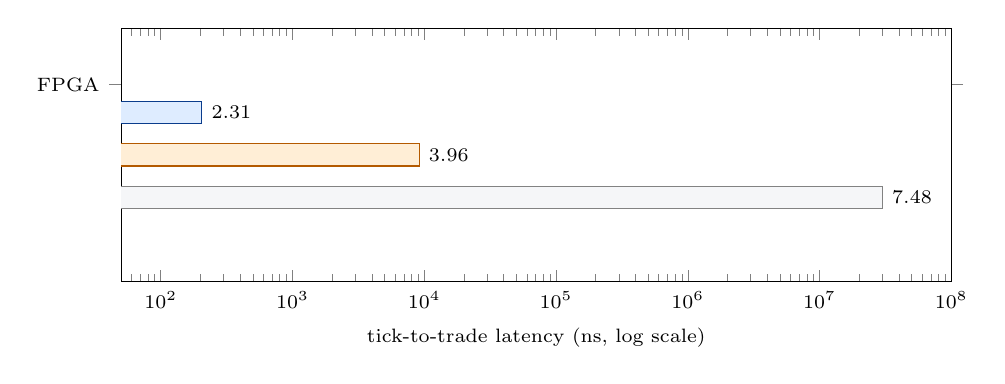
\begin{tikzpicture}
\begin{axis}[
  width=\linewidth, height=4.8cm,
  xbar, xmode=log, log basis x=10,
  xlabel={tick-to-trade latency (ns, log scale)},
  xlabel style={font=\scriptsize}, tick label style={font=\scriptsize},
  symbolic y coords={IBKR net,SW host,FPGA}, ytick=data,
  xmin=50, xmax=1e8, nodes near coords, every node near coord/.append style={font=\scriptsize},
  enlarge y limits=0.4, bar width=8pt,
]
\addplot[fill=hwfill, draw=hdrblue] coordinates {(205,FPGA)};
\addplot[fill=swfill, draw=warnamber] coordinates {(9149,SW host)};
\addplot[fill=tablegray, draw=rulegray] coordinates {(30000000,IBKR net)};
\end{axis}
\end{tikzpicture}\\[-1pt]
{\scriptsize\color{rulegray} FPGA 205\,ns (measured) vs.\ SW compute
$\approx$9\,$\mu$s vs.\ broker RTT $\approx$30\,ms.}
\end{minipage}

\smallskip
\textbf{Measured comparison (live AAPL soak):} FPGA \textbf{205\,ns} vs.\ software
compute \textbf{$\approx$9{,}149\,ns mean} on the same logic = $\sim$45$\times$ on
compute alone; once the live \emph{order} path adds network round-trip
($\sim$tens of ms), the end-to-end gap is $\sim$5 orders of magnitude. (See the
companion \fpath{why\_fpga\_beats\_cpu\_parallelism.pdf} for the deep dive.)

\newpage
% ── 5. File-by-file reference ───────────────────────────────────────────────────
{\large\bfseries\color{hdrblue} 5.\quad Every File, Explained}
\sectionrule

{\bfseries\color{hdrblue} RTL \textendash{} the hardware (\fpath{rtl/})}
\vspace{2pt}
\begin{center}\small
\renewcommand{\arraystretch}{1.2}
\begin{tabularx}{\linewidth}{@{}l X@{}}
\toprule
\textbf{File} & \textbf{What it does} \\
\midrule
\fpath{itch\_parser.sv}        & Decodes NASDAQ ITCH messages (Add/Cancel/Delete/Execute) into typed fields. Stage 1 of the pipeline. \\
\fpath{order\_book\_m2.sv}     & M2 order book: 256-slot direct-mapped table, IDLE/RESCAN FSM that recomputes best bid/ask after any cancel/delete/execute. \\
\fpath{order\_book\_top.sv}    & M1 reference book (top-of-book only); kept for comparison. \\
\fpath{strategy\_imbalance.sv} & Depth-weighted imbalance strategy, 2-stage pipeline, cross-multiply trigger, spread guard, cooldown, lot sizing. \\
\fpath{risk\_check.sv}         & Pre-trade risk: max order size, price band (fat-finger), net-position limit, kill switch (Rule 15c3-5 style). \\
\fpath{latency\_counter.sv}    & Hardware tick-to-trade timer + 64-bucket histogram, read over AXI-Lite. \\
\fpath{tick\_to\_trade\_top.sv}& Top level wiring parser$\to$book$\to$strategy$\to$risk$\to$output + latency counter. \\
\fpath{multi\_symbol\_book.sv} / \fpath{multi\_symbol\_top.sv} & 4-symbol scaled version (M2): replicated books behind a symbol mux/arbiter. \\
\fpath{top.xdc}                & Timing/pin constraints (200\,MHz clock, false-path AXI-Lite, I/O budget). \\
\bottomrule
\end{tabularx}
\end{center}

{\bfseries\color{accentteal} Golden models \textendash{} the Python oracle (\fpath{sim/golden/})}
\vspace{2pt}
\begin{center}\small
\renewcommand{\arraystretch}{1.2}
\begin{tabularx}{\linewidth}{@{}l X@{}}
\toprule
\textbf{File} & \textbf{What it does} \\
\midrule
\fpath{itch\_parser.py}      & Reference ITCH decoder. \\
\fpath{order\_book.py}       & M1 reference book. \\
\fpath{order\_book\_m2.py}   & Faithful M2 RESCAN book (256-slot, ref-aliasing, top-4 cache) --- the book oracle. \\
\fpath{strategy\_imbalance.py}& Faithful depth-weighted strategy mirror --- the strategy oracle. \\
\bottomrule
\end{tabularx}
\end{center}

{\bfseries\color{hdrblue} Simulation / verification (\fpath{sim/})}
\vspace{2pt}
\begin{center}\small
\renewcommand{\arraystretch}{1.25}
\begin{tabularx}{\linewidth}{@{}>{\raggedright\arraybackslash}p{5.4cm} X@{}}
\toprule
\textbf{File(s)} & \textbf{What it does} \\
\midrule
\fpath{tb\_itch\_parser.py}, \fpath{tb\_order\_book.py}, \fpath{tb\_order\_book\_m2.py}, \fpath{tb\_strategy\_imbalance.py}, \fpath{tb\_risk\_check.py}, \fpath{tb\_latency\_counter.py}, \fpath{tb\_tick\_to\_trade.py} & cocotb unit + integration testbenches: drive each RTL module in QuestaSim and assert its outputs match the golden models. \\
\fpath{tb\_multi\_symbol\_book.py}, \fpath{tb\_multi\_symbol\_top.py} & Multi-symbol scaling tests. \\
\fpath{tb\_replay\_regression.py} & Feeds generated ITCH; asserts book equivalence + reports strategy decisions (Phase 2). \\
\fpath{tb\_phase3\_pipeline.py} & Full-pipeline harness; reads the latency histogram over AXI-Lite (Phase 3). \\
\fpath{tb\_shadow\_quotes.py} & Feeds one quote stream to RTL \emph{and} software; diffs decisions $\to$ \fpath{reports/shadow\_report.csv}. \\
\fpath{tb\_cl\_csr.py} & Tests the F1 CL wrapper + CSR bridge (ITCH in / decisions out over one AXI-Lite). \\
\fpath{phase2\_golden.py} & Pure-Python parser\,$\to$\,book\,$\to$\,strategy\,$\to$\,risk runner. \\
\fpath{replay\_gen.py}, \fpath{synth\_itch.py} & Seeded ITCH generators / real-slice loader. \\
\fpath{pipeline\_sva.sv} & SystemVerilog assertions bound to the pipeline. \\
\fpath{Makefile} & cocotb/Questa build (\texttt{SIM=questa TOPLEVEL=\dots\ MODULE=\dots}). \\
\bottomrule
\end{tabularx}
\end{center}

{\bfseries\color{warnamber} Host / live trading (\fpath{host/})}
\vspace{2pt}
\begin{center}\small
\renewcommand{\arraystretch}{1.2}
\begin{tabularx}{\linewidth}{@{}l X@{}}
\toprule
\textbf{File} & \textbf{What it does} \\
\midrule
\fpath{strategy\_sw.py} & Bit-identical software mirror of \fpath{strategy\_imbalance.sv} (kept in sync with the golden model). \\
\fpath{risk\_guard.py}  & Software risk checks aligned to \fpath{risk\_check.sv} parameters. \\
\fpath{live\_feed.py}   & The live engine: Alpaca/IBKR quotes $\to$ strategy $\to$ risk $\to$ paper orders. Modes: \texttt{-{}-alpaca}, \texttt{-{}-symbol} (IBKR), \texttt{-{}-simulate}, \texttt{-{}-demo}; \texttt{-{}-execute} places real paper orders (IOC, with cancel-on-new + no-cross inventory clamp + broker-position sync). \\
\fpath{ibkr\_bridge.py} & IBKR order-routing bridge (dry-run / paper). \\
\fpath{quote\_sim.py}   & Synthetic continuous live-quote generator (shared by \texttt{-{}-simulate} and shadow tests). \\
\bottomrule
\end{tabularx}
\end{center}

{\bfseries\color{hdrblue} F1 deployment (\fpath{f1/}) \quad\&\quad Gate-level (\fpath{gatesim/})}
\vspace{2pt}
\begin{center}\small
\renewcommand{\arraystretch}{1.2}
\begin{tabularx}{\linewidth}{@{}l X@{}}
\toprule
\textbf{File} & \textbf{What it does} \\
\midrule
\fpath{cl\_tick\_to\_trade\_core.sv} & Custom-Logic wrapper: CSR bridge + core behind one OCL AXI-Lite (sim-validated). \\
\fpath{cl\_tick\_to\_trade.sv}      & AWS Shell port template for the AFI build. \\
\fpath{register\_map.md}            & AXI-Lite address map, m\_axis decision format, risk reason codes. \\
\fpath{host\_replay.py}             & Offline golden self-check + \texttt{-{}-device} stub for F1 readback. \\
\fpath{gen\_netlist.tcl}, \fpath{compile\_simlib.tcl}, \fpath{*\_funcsim.v} & Gate-level (post-synthesis) netlist + sim-lib for functional gate simulation. \\
\bottomrule
\end{tabularx}
\end{center}

{\bfseries\color{accentteal} Docs (\fpath{docs/}) \quad\&\quad Notebooks / reports}
\vspace{2pt}
\begin{center}\small
\renewcommand{\arraystretch}{1.2}
\begin{tabularx}{\linewidth}{@{}l X@{}}
\toprule
\textbf{File} & \textbf{What it does} \\
\midrule
\fpath{part1/2/3\_*.tex} & Three-part learning series: foundation/architecture, RTL design \& verification, integration \& deployment. \\
\fpath{implementation\_results.tex} & Measured Vivado results (LUTs, timing/WNS, power) for both designs. \\
\fpath{validation\_roadmap.tex} & The 4-phase validation plan (timing $\to$ sim regression $\to$ F1 $\to$ live). \\
\fpath{live\_execution\_issues.tex} & Every real-broker issue hit in live paper trading + fixes. \\
\fpath{why\_fpga\_beats\_cpu\_parallelism.tex} & Spatial/pipeline parallelism deep dive. \\
\fpath{executive\_summary.tex}, \fpath{issues\_log.tex} & One-page summary; running issues log. \\
\fpath{notebooks/latency\_histogram*.ipynb} & Latency charts (FPGA vs IBKR, per-message, histogram, scorecard). \\
\fpath{reports/shadow\_report.csv}, \fpath{reports/soak\_aapl.log} & FPGA-vs-SW equivalence CSV; live-soak capture. \\
\bottomrule
\end{tabularx}
\end{center}

% ── 6. End-to-end flow ──────────────────────────────────────────────────────────
{\large\bfseries\color{hdrblue} 6.\quad End-to-End Flow \textendash{} Bench to Silicon to Live}
\sectionrule

\begin{center}
\resizebox{0.95\linewidth}{!}{%
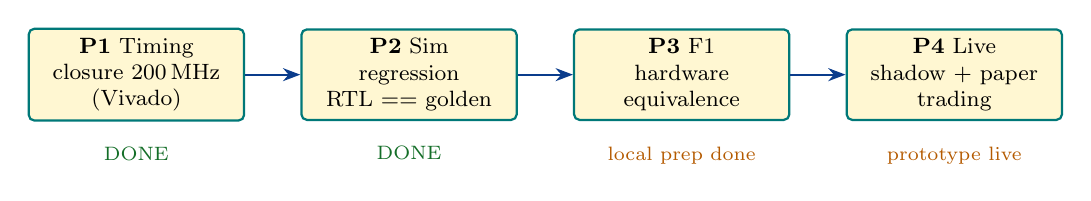
\begin{tikzpicture}[node distance=4mm and 7mm]
\node[gold] (p1) {\textbf{P1} Timing\\ closure 200\,MHz\\ (Vivado)};
\node[gold, right=of p1] (p2) {\textbf{P2} Sim\\ regression\\ RTL == golden};
\node[gold, right=of p2] (p3) {\textbf{P3} F1\\ hardware\\ equivalence};
\node[gold, right=of p3] (p4) {\textbf{P4} Live\\ shadow + paper\\ trading};
\foreach \x/\y in {p1/p2,p2/p3,p3/p4} \draw[flow] (\x) -- (\y);
\node[below=2mm of p1, font=\scriptsize, text=okgreen] {DONE};
\node[below=2mm of p2, font=\scriptsize, text=okgreen] {DONE};
\node[below=2mm of p3, font=\scriptsize, text=warnamber] {local prep done};
\node[below=2mm of p4, font=\scriptsize, text=warnamber] {prototype live};
\end{tikzpicture}}
\end{center}

\textbf{The verification invariant} (true at every phase): \emph{feed identical
input to the FPGA and to the Python golden model; assert the decisions match.}
Only the input fidelity and the execution substrate change --- synthetic in P1/P2,
real silicon in P3, real market data in P4. This is what lets a 205\,ns hardware
number and a live paper trade be the \emph{same strategy}, just realised
differently.

\vfill
{\small\color{rulegray} Companion documents: \fpath{part1/2/3\_*.pdf} (tutorial
series), \fpath{implementation\_results.pdf} (measured timing/area/power),
\fpath{validation\_roadmap.pdf} (phase plan), \fpath{live\_execution\_issues.pdf}
(live-trading issues), \fpath{why\_fpga\_beats\_cpu\_parallelism.pdf}. Build:
\texttt{pdflatex project\_complete\_flow.tex}.}

\end{document}
